
%%% Local Variables: 
%%% mode: latex
%%% TeX-master: t
%%% End: 

\chapter{凸包围体生成算法}
\label{cha:kcbp-construction}
从\ref{sec:convex-bv}可以看出包围体的紧致程度直接影响算法的效率,对于不规则形体, 常见的包围体往往不够紧致,凸包紧致但往往包含过多的面片数而增加算法的复杂性。

本文提出一种构造凸包围多面体的方法,该方法首先利用近似内凸包和~$k$-means~聚类算法生成构成凸包围多面体~$k$~个截面的法向。
然后根据输入点集沿各法向搜索切点构成截面, 最后由这些截面通过对偶映射的方式求交构成凸包围多面体。
该方法的主要优势是:
\begin{inparaenum}[1)]
\item 对给定点集可构造紧致的包围体;
\item 利用~GPU~加速,能够快速构造包围体;
\item 通过参数~$k$~调节凸包围多面体的简单性和紧致性,可适用于不同的应用场景。
\end{inparaenum}

由~$k$~个截面构成的凸包围多面体称为凸包围~$k$~面体($k$-Convex Bounding Polytope, 简称~$k$-CBP), 可通过~$k$~个半空间定义:
\begin{equation}
\label{equ:kcbp_definition}
\left\{
\begin{array}{l}
    k\mbox{-CBP} = \mathop  \bigcap \limits_{i = 1}^k \bm{H_i} \\
    \bm{H_i} = \left\{ {\left. {\bm{p} \in {\mathbb{R}^3}} \right| \bm{n_i} \cdot \bm{p} \le {w_i}} , w_i \in \mathbb{R} \right\},
\end{array}
\right.
\end{equation}

其中,$\bm{n_i}$~是半空间~$\bm{H_i}$~的法向,方向指向包围体外部,
$w_i$~是输入点集中沿~$\bm{n_i}$~方向投影的最大值。
如图\ref{fig:bunny}所示是~Bunny~模型的凸包围~34~面体(34-CBP)。

\begin{figure}[H] 
\centering
  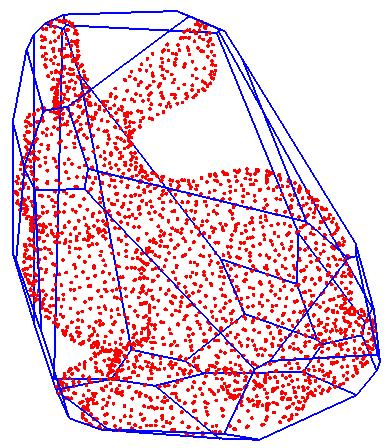
\includegraphics[width=1.3in]{bunny-34.png}
  \caption{~Bunny~模型的~34-CBP }
  \label{fig:bunny}
\end{figure}

本文提出的算法主要流程如图~\ref{lbl:kcbp-algorithm-flowchart}~
所示,首先利用近似内凸包和~$k$-means~聚类算法生成构成凸包围多面体~$k$~个截面的法向,然后根据输入点集在~GPU~中沿各法向搜索切点构成截面,
最后由这些截面通过对偶映射的方式求交构成凸包围多面体。搜索截面需要多次扫描输入点集,在~CPU~中计算较耗时,因此用~GPU~加速使得算法整体性能得以提升,其他步骤在~CPU~计算即可。

\begin{figure}[H]
    \centering
    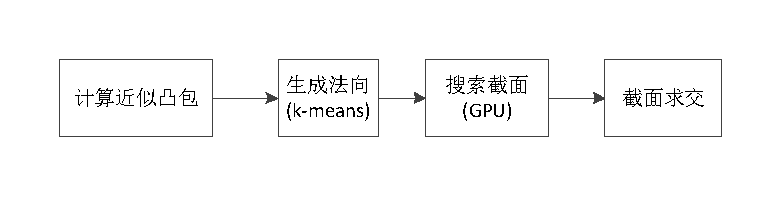
\includegraphics[height=0.7in]{kcbp-flowchart-x-aix.pdf}
    \caption{算法流程图}
    \label{lbl:kcbp-algorithm-flowchart}
\end{figure}

图\ref{lbl:bunny-26-cbp-ch-ach}~
从左至右分别显示了~Bunny~模型的~26-CBP、精确凸包和近似内凸包。近似凸包是精确凸包的一种近似,与精确凸包外观相似但其构造复杂度降低,不少研究者利用该性质解决计算机图形学中很多问题
\cite{hossain2013constructing}。本文就是利用近似内凸包与精确凸包的相似性,从众多近似凸包面片的法向中通过聚类算法生成凸包围多面体的~$k$~个法向。
%由图可知, 近似内凸包的三角面片大致反映了精确凸包三角面片的分布情况,近似内凸包相应位置面积较大的三角面片对应到精确凸包的三角面片面积也较大, 因此该三角面片所在平面需尽量保留.
\begin{figure}[H] % use [h] to fix the position
\centering
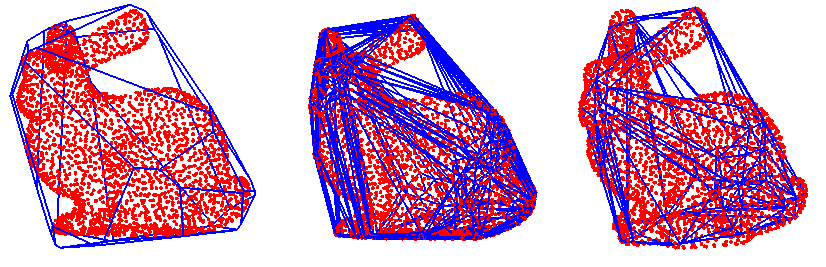
\includegraphics[width=5.0in]{26-bunny-ach-ch-kcbp.png}
\caption{~Bunny~模型的~26-CBP、凸包和近似内凸包}
\label{lbl:bunny-26-cbp-ch-ach}
\end{figure}
本章将按步骤详细介绍算法的实现。

\section{截面法向的生成}
\label{sec:gen-normals}

截面法向的选定与多面体的紧致程度密切相关。
$k$-DOP预先定义~$k/2$对法向,且$k$值局限于6、14、18或26等少数几个,导致其生成的多面体不能自适应模型,对于不规则形体不够紧致。相比本文$k$值取值更灵活,因此可以根据不同需求不同应用场景更加灵活地计算出凸包围体。
根据经验,为了使凸包围多面体尽可能逼近凸包,在多面体数量一定的情况下需尽量保留凸包中面积较大的面。 
本文算法先通过一种线性算法\cite{bentley1982approximation}构造近似内凸包,然后从近似内凸包里选取面积最大的~$a$~个面的法向,最后用聚类算法从剩下的面中生成~$k-a$~个法向。

\subsection{近似内凸包生成聚类样本法向集}
\label{subsec:ach-gen-normals}

下面以平面点集的近似内凸包为例说明初始法向集的生成。
\begin{figure}[H]
  \centering
  \subcaptionbox{Place points in bin\label{lbl:subfig-split-groups}}{
    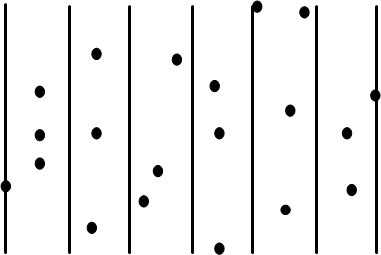
\includegraphics[width=1.7in]{approximate-convexhull-step1.png}} \hspace{0.5cm}
  \subcaptionbox{Find extremes in bins \label{lbl:subfig-find-extrems}}{%
    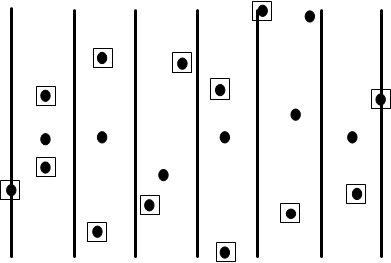
\includegraphics[width=1.7in]{approximate-convexhull-step2.png}} \hspace{0.5cm}
  \subcaptionbox{Choose extremes to build approximate hull\label{lbl:subfig-connect-extremes}}{%
    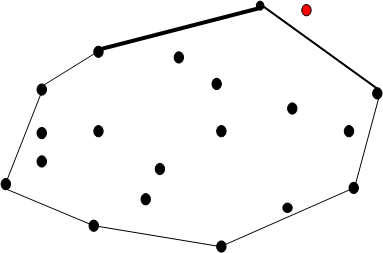
\includegraphics[width=1.7in]{approximate-convexhull-step3.png}} \hspace{0.5cm}
  \caption{二维近似内凸包的构造\cite{bentley1982approximation}}
\label{lbl:ach-2d}
\end{figure}

如图\ref{lbl:ach-2d}所示,整个算法分为3个步骤:
\begin{inparaenum}[(1)]
\item \textbf{分组。}
首先根据~$x$~轴将输入点均分~$\xi$~组,如图\ref{lbl:subfig-split-groups}所示,$\xi$值可以根据输入点集数量以及希望得到的近似凸包的近似程度进行选取,图示中分成了6组。
\item \textbf{选极值点。}
然后在每组中找出沿~$y$~轴的最大最小值,得到每组的极值点,如图\ref{lbl:subfig-find-extrems}所示,在边界上的点可直接当作极值点。
\item \textbf{连线。}
最后按条件连接每组的最值构成近似内凸包,如图\ref{lbl:subfig-connect-extremes}所示。//TODO,可更详细
\end{inparaenum}
此算法复杂度为~$O(n+\xi)$。  
得到近似凸包后,因较长的边(图中的粗边)对最后凸包围多边形影响较大, 因此可以保留较长的$a$条边(2D 为例), 其他$n-a$(n为近似内凸包边数)进行聚类得到$k-a$ 类, 最后得到边对应的垂直向外的方向作为法向。
在三维空间里, 可按照~$x,y$~轴最多划分成 $(\xi+2)\times (\xi+2)$个网格, 每个网格取~$z$~的最大最小值, 因此所有网格含最多有~$2(\xi+2)^2$~个极值点, 其凸包可以在$O(\xi^2\log \xi^2) = O(\xi^2\log \xi)$ 内找出, 因此整个算法时间复杂度为$O(n+\xi^2\log\xi)$, 
关于此算法更详细的细节可参考文献\onlinecite{bentley1982approximation}。 实验过程中, 为了更快地构造近似内凸包, $\xi$~值通常取得较小(例如取~$\xi=10$)。

假设点~$A,B,C$~为近似凸包的某个平面$P_i$上逆时针方向上的3个顶点,则该平面~$P_i$的法向$\bm{n_i}
= \overrightarrow{AB} \times
\overrightarrow{AC}$,这些法向就是参与聚类算法的所有样本法向集。


\subsection{聚类初始点的选择}
\label{subsec:initial-normals}

聚类算法是数据挖掘领域里的研究热点之一,$k$-means~是最流行和最简单的基于划分的聚类算法\cite{Jain2010}。其中,$k$-means
算法最初的步骤就是初始聚类中心的选择。本文算法将采取如下的策略生成:给定一个单位球,将其按照等面积划分成$k$份即$k$-means中的参数$k$,连接球心到每份中心点构成的方向作为法向,其效果如图\ref{lbl:kmeans-init-normals-26}所示($k=26$)。

\begin{figure}[H]
    \centering
    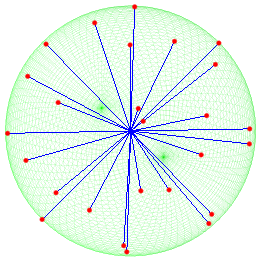
\includegraphics[height=1.7in]{kmeans-init-normals-26.png}
    \caption{初始聚类法向的生成}
    \label{lbl:kmeans-init-normals-26}
\end{figure}

初始点生成算法具体如~Algorithm\ref{alg:get_init_normals_by_area}~所示。另外,亦可使用如文献\onlinecite{wong1997sampling}中的数学统计方法在球面上生成若干个点使其满足均匀分布。

\begin{algorithm}[H]
\algsetup{linenosize=\tiny}
\small
\caption{初始法向的生成}
\label{alg:get_init_normals_by_area}
\begin{algorithmic}[1]
\REQUIRE
初始法向数量:$k$
\ENSURE
~$k$~个法向:Normal
\STATE $i \gets 0$; $area \leftarrow 4\pi / k$
\STATE $m\_v \gets round(\pi/\sqrt{area})$
\STATE $d\_v \gets \pi/m\_v$
\STATE $d\_phi \gets area/d\_v$
\FOR {$m=0$ \TO $m\_v-1$}
    \STATE $v \gets \pi m/m\_v$
    \STATE $m\_phi \gets round(2\pi\sin{v}/d\_phi)$
    \FOR {$n=0$ \TO $m\_phi-1$}
        \STATE $\phi \gets 2\pi n/m\_phi$
        \STATE $Normal_i \gets vec3(\sin{v}\cos{\phi},\sin{v}\sin{\phi},\cos{v})$
        \STATE $i \gets i+1$
    \ENDFOR
\ENDFOR
\RETURN $Normal$
\end{algorithmic}
\end{algorithm}

 
\subsection{聚类确定法向}
\label{subsec:determ-normals}

聚类算法将相似程度高的变量聚集到一类,距离度量是$k$-means中的关键,采用不同的距离计算函数可能得到不同的聚类结果,依据数据的不同性质可选用不同的距离度量方法,常用的有欧式距离,曼哈顿距离和卡方距离等等。
本文采用余弦距离度量,将方向相近的点归聚到一类。$k$-means~本质上是一个迭代贪心算法,每一次迭代需要重新计算每一类的中心点,直到两次迭代后中心点相差在预定的容差范围内为止。
本文聚类更新中心点时将面片的面积作为权重即
\begin{equation}
\label{equ:kmeans-update-center}
\bm{c_i}=\frac{\sum_{i=1}^{i=n} \omega_i \cdot \bm{n_i} } {\sum_{i=1}^{i=n} \omega_i}
,
\end{equation}
其中$\bm{c_i}$
为第~$i$~类的中心点,$\omega_i$~为法向~$\bm{n_i}$~所在面片对应的面积,这样使得生成的法向尽量靠近原始近似凸包面积较大的面片的方向。完整的算法如~Algorithm~\ref{alg:kmeans-determine-normals}所示。

\begin{algorithm}
\algsetup{linenosize=\tiny}
\small
\caption{$k$-means确定法向}
\label{alg:kmeans-determine-normals}
\begin{algorithmic}[1]
\REQUIRE
初始中心点 $init$, 聚类数量 $k$, 聚类样本法向集 $points$
\ENSURE
~$k$~个聚类后的法向 $result$

\FORALL {$p \in points$}
    %\STATE $tmp \gets -\infty $
    \FORALL {$c \in init$}
        \STATE $\phi \gets c \cdot p$ \COMMENT{计算余弦距离, 并记录每个聚类变量属于哪一类}
        %\STATE $tmp \gets max(tmp, \phi)$ \COMMENT{记录每个聚类变量属于哪一类}
    \ENDFOR
    \FORALL {$c \in init$}
        \STATE $result \gets update(c)$ \COMMENT{按照公式\ref{equ:kmeans-update-center}更新中心点}
    \IF{$chk\_state(result, init, iter)$}
        \RETURN {$result$}
        \COMMENT{检测迭代条件是否满足,中心点容差范围内不在变化或迭代次数超过最大迭代次数}
    \ELSE
        \STATE $init \gets result $
        \STATE $iter \gets iter+1 $
    \ENDIF
    \ENDFOR
\ENDFOR
\end{algorithmic}
\end{algorithm}


通过聚类后得到的法向生成包围体比直接用初始法向生成的包围体更加紧致。如图~\ref{lbl:kemans-fixed-kcbp}~所示, 
其中图~\ref{lbl:fixed-kcbp-bunny}~为按照初始方向为~Bunny~模型生成的凸包围多面体($k=26$),
聚类后其法向及其生成的凸包围多面体如图~\ref{lbl:kmeans-kcbp-bunny}~所示, 后者的紧致程度比前者高~14.98\%.

\begin{figure}[H]
\setcounter{subfigure}{0}
  \centering
  \subcaptionbox{初始法向生成$k$-CBP\label{lbl:fixed-kcbp-bunny}}{%
    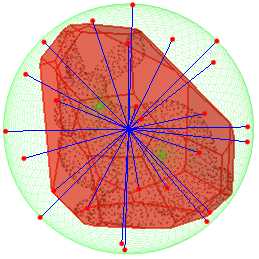
\includegraphics[width=1.8in]{kmeans-init-normals-26-for-bunny.png}}\hspace{3em}%
  \subcaptionbox{聚类法向生成$k$-CBP\label{lbl:kmeans-kcbp-bunny}}{%
    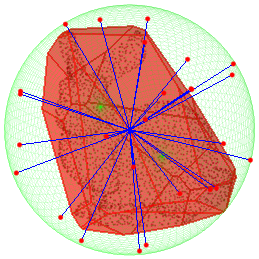
\includegraphics[width=1.8in]{kmeans-cluster-normals-26-for-bunny.png}}\hspace{3em}%
  \caption{初始法向和聚类确定法向生成$k$-CBP对比($k=26$)}
  \label{lbl:kemans-fixed-kcbp}
\end{figure}

\section{搜索截面}
\label{sec:search-planes}

\subsection{串行算法}
\label{subsec:determ-normals}


\subsection{基于~OpenGL Shader~的并行算法}
\label{subsec:determ-normals}

\subsection{基于~Cuda~的并行算法}
\label{subsec:determ-normals}


\section{截面求交算法}
\label{sec:intersect-planes}

\subsection{几何枚举算法}
\label{subsec:intersection-enum-geometry}

\subsection{对偶映射算法}
\label{subsec:intersection-dual-mappint}

\section{实验结果}
\label{sec:exper-kcbp}
